\section{App}
Die App soll den Features entsprechend schlicht gehalten werden.
So können wir die Nutzung der App intuitiv, einfach und schnell gestalten.
Der Benutzer soll sofort wissen wie er die App nutzen kann ohne eine entsprechende Einweisung.

\begin{figure}[ht]
	\centering
	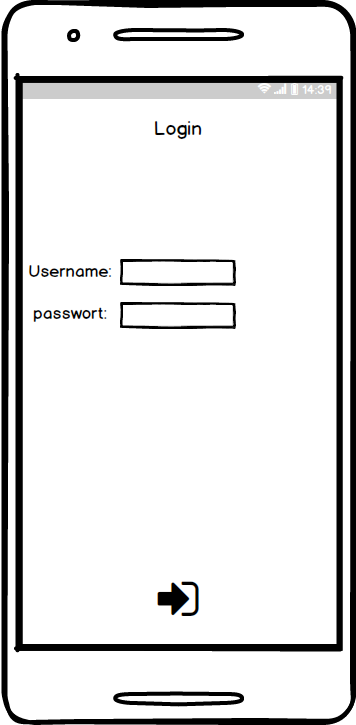
\includegraphics[keepaspectratio,width=5cm]{img/Login}
	\caption{Schlichte Login Seite}
	\label{fig:App1}
\end{figure}

\begin{figure}[ht]
	\centering
	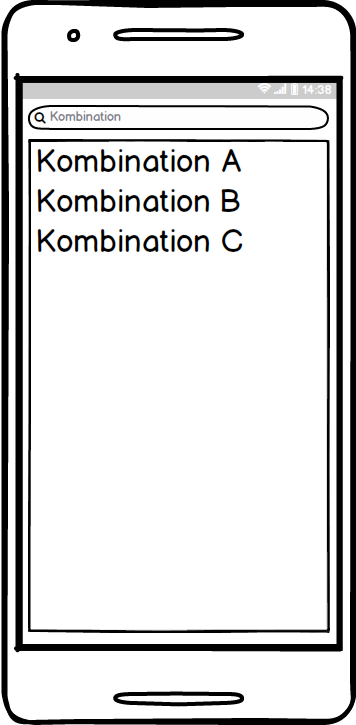
\includegraphics[keepaspectratio,width=8cm]{img/Kombination_suchen}
	\caption{Suchen nach gespeichterten Kombinationen}
	%\label{fig:mock-pw}
\end{figure}

\begin{figure}[ht]
	\centering
	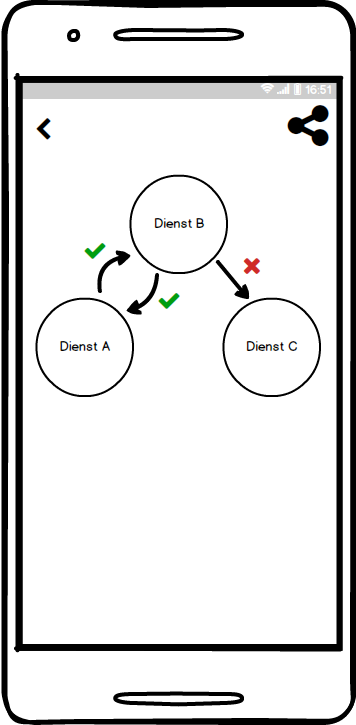
\includegraphics[keepaspectratio,width=8cm]{img/Kombination_anzeigen_Verbunden}
	\caption{Anzeigen einer Kombination}
	%\label{fig:mock-pw}
\end{figure}

\begin{figure}[ht]
	\centering
	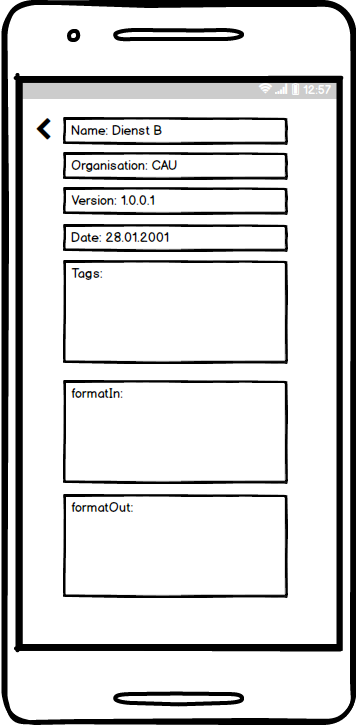
\includegraphics[keepaspectratio,width=8cm]{img/Dienst_anzeigen_Dienst_B}
	\caption{Darstellung eines einzelnen Dienstes}
	%\label{fig:mock-start}
\end{figure}

\begin{figure}[ht]
	\centering
	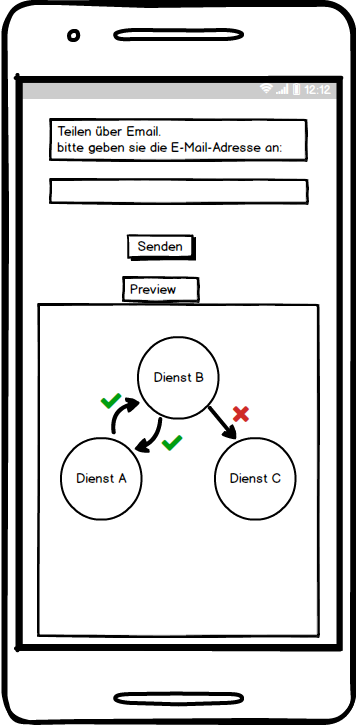
\includegraphics[keepaspectratio,width=8cm]{img/Kombination_teilen}
	\caption{Mögliches Teilen per Email einer Kombination}
	%\label{fig:mock-pw}
\end{figure}

\section{Webseite}
Auf der Webseite können von jedem Benutzer Dienstkombinationen angelegt und bearbeitet werden.
Diese Kombinationen werden gespeichert und ggf. für weitere Benutzer freigegeben.
Das Verknüpfen von jeweils zwei Diensten geschieht mittels Drag \& Drop.
Sollten miteinander verknüpfte Dienste nicht kompatibel zueinander sein, kann die Software alternative Vorschläge anzeigen, um diese Inkompatibilität aufzulösen.
Zusätzlich dürfen Administratoren Dienste und Eingabe- bzw. Ausgabeformate verwalten.
Eine einfache Benutzerverwaltung soll ebenfalls eingebaut werden, die es Administratoren erlaubt,
Benutzern Administratorenrechte zu geben oder wieder zu entziehen.
Obwohl die Webseite deutlich komplexer sein wird als die App, soll auch hier der Fokus auf Benutzerfreundlichkeit und einer intuitiven Bedienung gesetzt werden. Auch ohne Einweisung soll es dem Benutzer schnell gelingen, beliebige Kombinationen von Diensten zu erstellen.

\begin{figure}[ht]
	\centering
	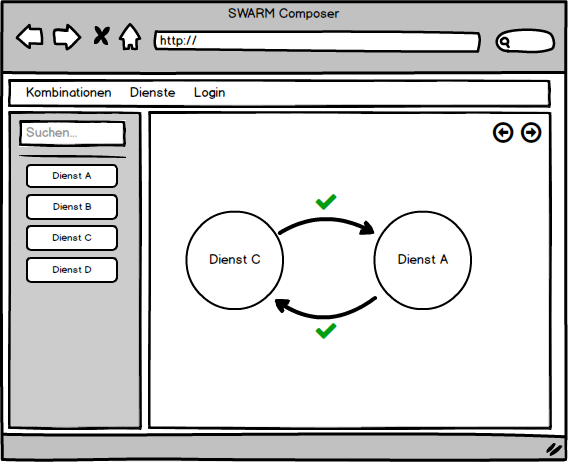
\includegraphics[keepaspectratio,width=11cm]{img/webfrontend/Kombinationen_Detail_Anonym.png}
	\caption{Darstellung einer Kombination ohne Account.}
	%\label{fig:mock-web-combination}
\end{figure}

\begin{figure}[ht]
	\centering
	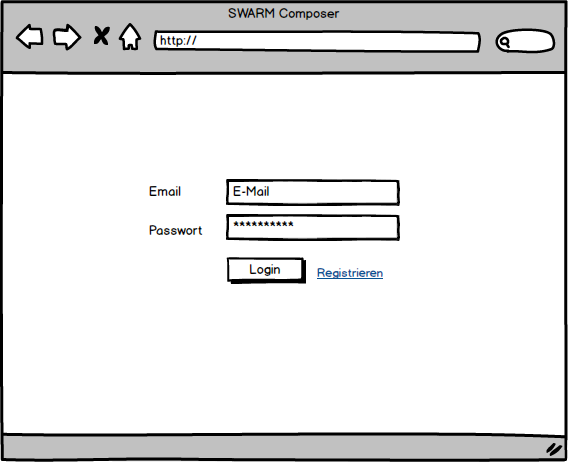
\includegraphics[keepaspectratio,width=11cm]{img/webfrontend/Login.png}
	\caption{Login}
	%\label{fig:mock-web-login}
\end{figure}

\begin{figure}[ht]
	\centering
	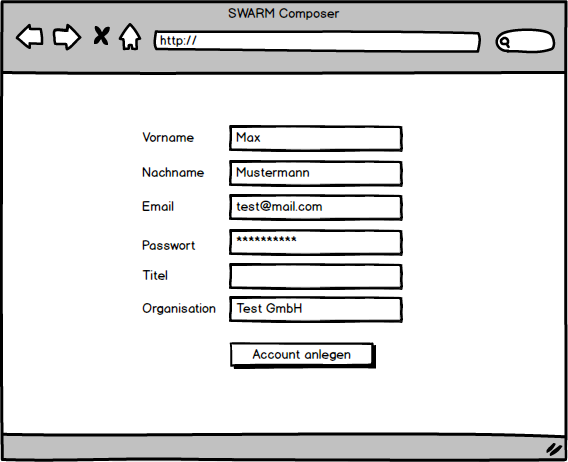
\includegraphics[keepaspectratio,width=11cm]{img/webfrontend/Registrieren.png}
	\caption{Neuen Account erstellen}
	%\label{fig:mock-web-register}
\end{figure}
\begin{figure}[ht]
	\centering
	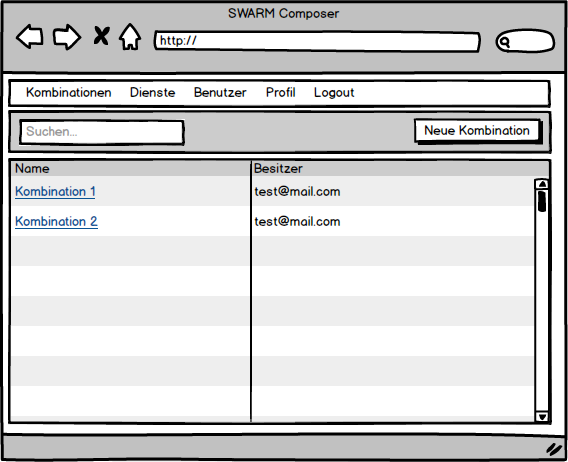
\includegraphics[keepaspectratio,width=11cm]{img/webfrontend/Kombinationen.png}
	\caption{Auflistung der Dienstkombinationen}
	%\label{fig:mock-web-combinations}
\end{figure}

\begin{figure}[ht]
	\centering
	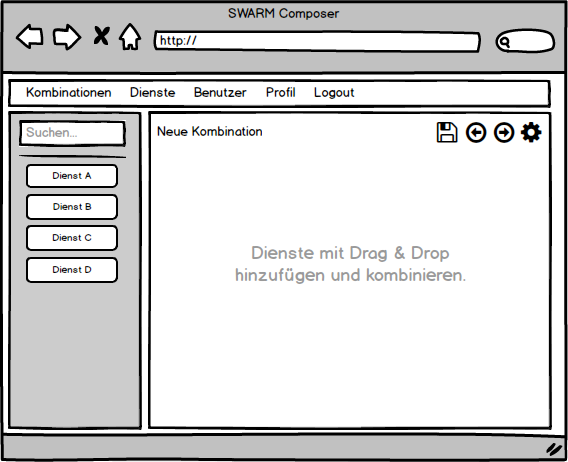
\includegraphics[keepaspectratio,width=11cm]{img/webfrontend/Kombinationen_Leer.png}
	\caption{Eine leere Kombination ohne Dienste}
	%\label{fig:mock-web-emptycombination}
\end{figure}

\begin{figure}[ht]
	\centering
	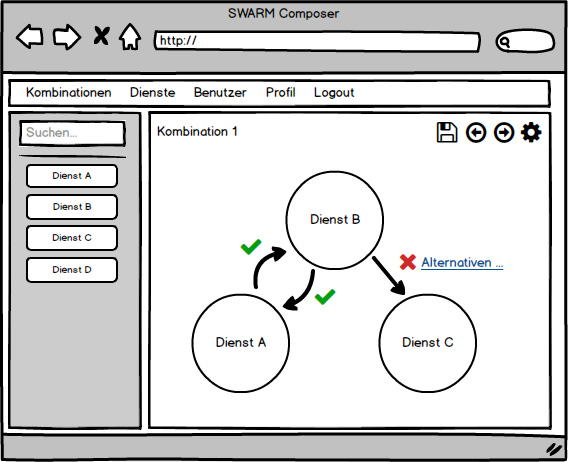
\includegraphics[keepaspectratio,width=11cm]{img/webfrontend/Kombinationen_Detail.png}
	\caption{Eine Kombination, die mehrere Dienste miteinander verknüpft. 'Dienst B' und 'Dienst C' sind inkombatibel}
	%\label{fig:mock-web-combination}
\end{figure}

\begin{figure}[ht]
	\centering
	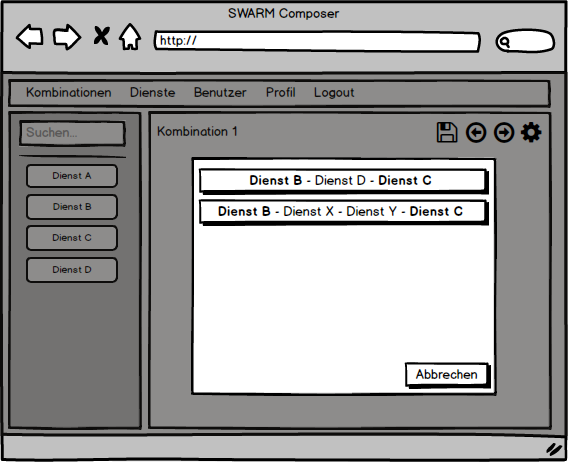
\includegraphics[keepaspectratio,width=11cm]{img/webfrontend/Kombinationen_Alternativen.png}
	\caption{Alternativen zu inkompatiblen Diensten}
	%\label{fig:mock-web-alternatives}
\end{figure}

\begin{figure}[ht]
	\centering
	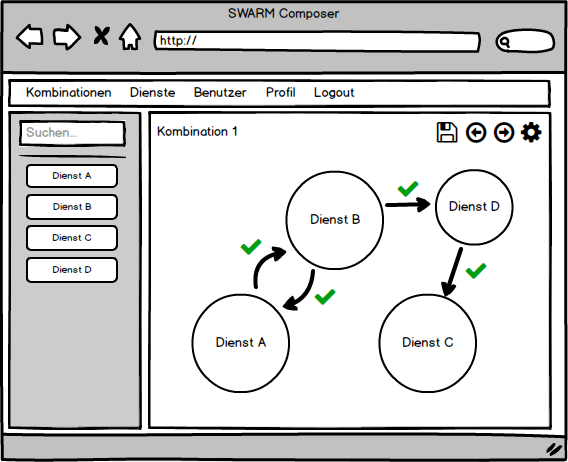
\includegraphics[keepaspectratio,width=11cm]{img/webfrontend/Kombinationen_Details_Neu.png}
	\caption{Alternative Dienste werden automatisch eingefügt}
	%\label{fig:mock-web-combinationalt}
\end{figure}

\begin{figure}[ht]
	\centering
	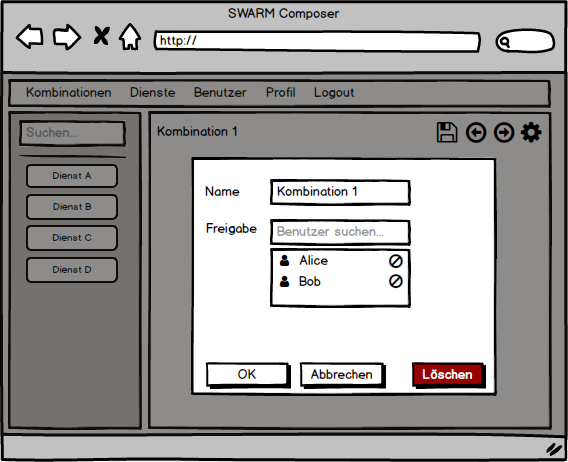
\includegraphics[keepaspectratio,width=11cm]{img/webfrontend/Kombinationen_Optionen.png}
	\caption{Details zu einer Kombination}
	%\label{fig:mock-web-combinationdialog}
\end{figure}

\begin{figure}[ht]
	\centering
	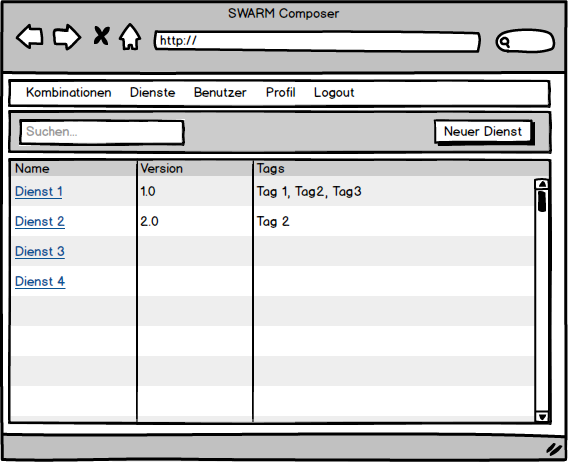
\includegraphics[keepaspectratio,width=11cm]{img/webfrontend/Dienste.png}
	\caption{Auflistung der Dienste}
	%\label{fig:mock-web-services}
\end{figure}

\begin{figure}[ht]
	\centering
	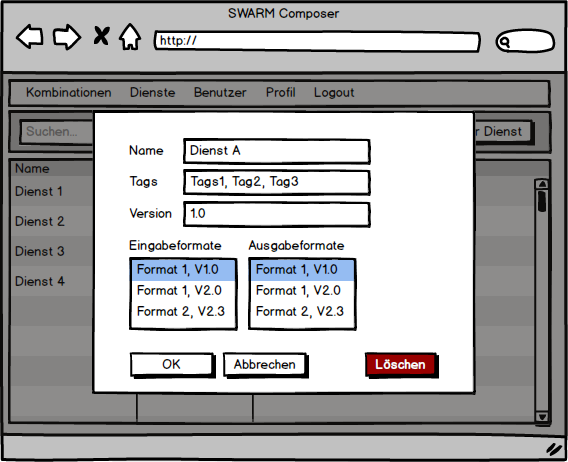
\includegraphics[keepaspectratio,width=11cm]{img/webfrontend/Dienste_Detail.png}
	\caption{Details zu einem Dienst}
	%\label{fig:mock-web-servicedetail}
\end{figure}

\begin{figure}[ht]
	\centering
	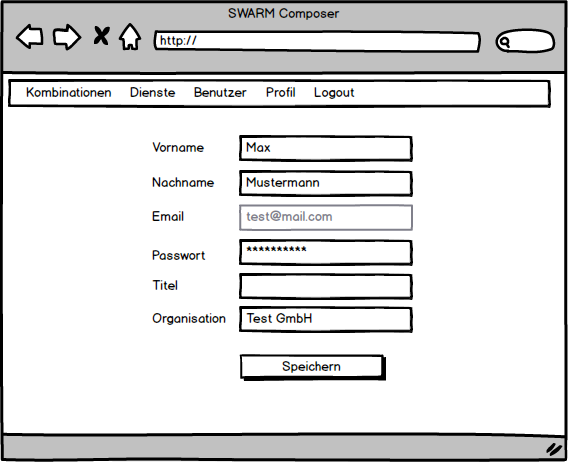
\includegraphics[keepaspectratio,width=11cm]{img/webfrontend/Profil.png}
	\caption{Benutzer können ihre gespeicherten Daten einsehen und ändern.}
	%\label{fig:mock-web-formats}
\end{figure}

\begin{figure}[ht]
	\centering
	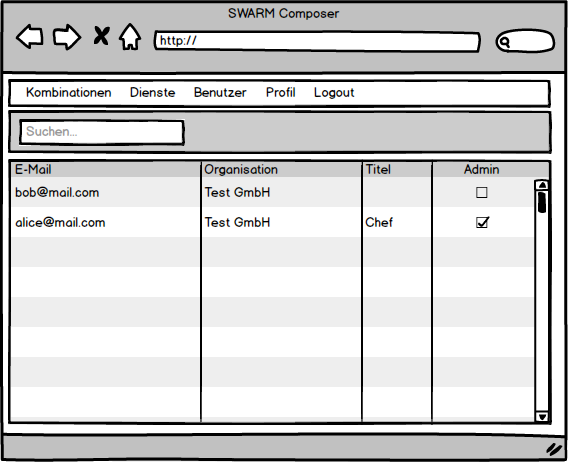
\includegraphics[keepaspectratio,width=11cm]{img/webfrontend/Benutzer.png}
	\caption{Auflistung der Benutzer.}
	%\label{fig:mock-web-users}
\end{figure}
